\section{Mis primeros shader de juguete}
\begin{frame}{Repositorio}
Todo lo necesario para este taller esta en este repositorio: 
\begin{block}{}
\url{https://github.com/nemediano/tallerShadertoy}.
\end{block}
\begin{itemize}
    \item Ésta presentación, también esta en el mismo repositorio. Así puedes seguir los links.
    \item Para cada ejercicio, hay dos versiones de código fuente.
    \begin{enumerate}
        \item El código mínimo para empezar el ejercicio
        \item Una posible solución al ejercicio 
    \end{enumerate}
\end{itemize}

\end{frame}

\begin{frame}{Últimos detalles}
En shadertoy, la ejecución inicia y termina con la función:

\mintinline{glsl}{void mainImage(out vec4 fragColor, in vec2 fragCoord)}.

\begin{itemize}
    \item Por cada fragment recibes de parámetro: \mintinline{glsl}{fragCoord}, con la posición del fragment en el \emph{render target}.
    \item La salida: \mintinline{glsl}{fragColor}, es un output parameter. Un vector de dimensión 4 que debe contener el color final del fragment.
    \begin{itemize}
        \item La salida $\mathbf{x} \in \mathbb{R}^{4}$ debe tener $ x_i \in [0, 1]$.
        \item El último componente $x_4$ (ó bien $w$), representa el componente alpha, que en Shadertoy debe ser 1.
    \end{itemize}
\end{itemize}
\end{frame}

\begin{frame}{Bandera a cuadros}
    \begin{columns}
\column[t]{0.5\textwidth}
     \begin{itemize}
         \item Tratar de escribir un shader que genere una bandera a cuadros (o tablero de ajedrez si lo prefieres)
         \item Puedes empezar con el código de default de shader toy.
         \item Recuerda las funciones trigonométricas
     \end{itemize}
\column[t]{0.5\textwidth}
        \begin{figure}[htb]
            \centering
            
\includegraphics[width=0.6\textwidth]{img/Ejer1}
            \caption{\url{https://github.com/nemediano}}
        \end{figure}
\end{columns}
\end{frame}


\subsection{Funciones de distancia}

\begin{frame}{Sistema de coordenadas}
\begin{columns}
\column[t]{0.5\textwidth}
    \begin{itemize}
         \item Al principio, las coordenadas del fragment están en el espacio del imagen del render target. Miden pixeles.
         \item Cuando dividimos entre la resolución del render target, están en coordenadas de textura ($uv$-mapping). $u,v \in [ 0,1 ]$
     \end{itemize}
\column[t]{0.5\textwidth}
\begin{figure}[htp]
 \centering
 \begin{subfigure}[b]{0.45\textwidth}
   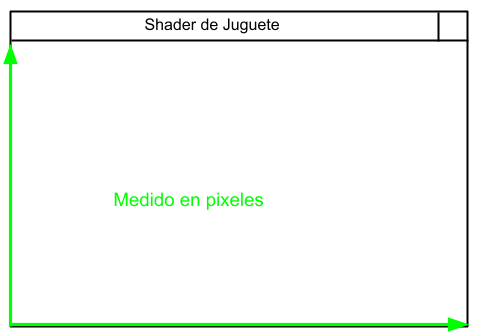
\includegraphics[width=\textwidth]{img/FrameOfreference}
   \caption{Espacio de imagen}
 \end{subfigure}
\\
 \begin{subfigure}[b]{0.45\textwidth}
   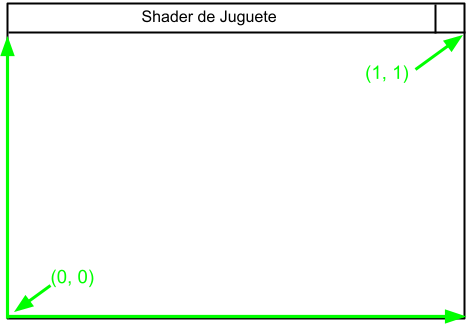
\includegraphics[width=\textwidth]{img/FoRUVSpace}
   \caption{$uv$ space}
 \end{subfigure}
\end{figure}
\end{columns}
\end{frame}

\begin{frame}{Sistema de coordenadas II}
\begin{columns}
\column[t]{0.5\textwidth}
    \begin{itemize}
        \item Cuando restamos 0.5 y multiplicamos por dos. Están en coordenadas normalizadas. $x,y \in [-1, 1]$.
        \item Cuando corregimos con el \emph{aspect ratio} de la pantalla, están en coordenadas de la escena. El origen esta en el centro, el eje mas restrictivo esta en $[-1, 1]$ y el otro es proporcional.
     \end{itemize}
\column[t]{0.5\textwidth}
\begin{figure}[htp]
 \centering
 \begin{subfigure}[b]{0.45\textwidth}
   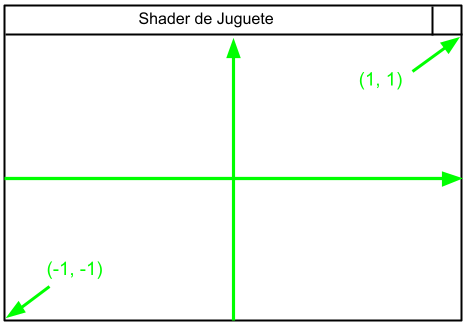
\includegraphics[width=\textwidth]{img/FoRNormalized}
   \caption{Normalize coordinates}
 \end{subfigure}
\\
 \begin{subfigure}[b]{0.45\textwidth}
   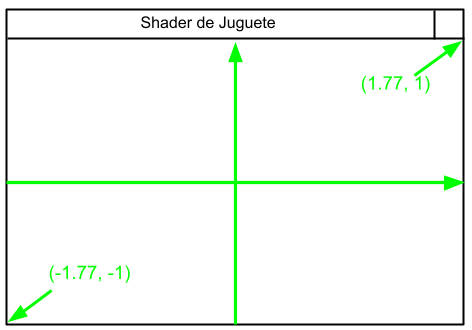
\includegraphics[width=\textwidth]{img/FoRCorrected}
   \caption{World Coordinates}
 \end{subfigure}
\end{figure}
\end{columns}
\end{frame}

\begin{frame}[fragile]{Función de transformación}
\begin{listing}
\begin{minted}{glsl}
vec3 getWorldCoordinates(vec2 fragCoord) {
    // UV coordinates
    vec2 uv = fragCoord/iResolution.xy;
    // Normalized coordinates
    vec2 norm = 2.0 * (uv - vec2(0.5));
    // World coordinates
    float aspectRatio = iResolution.x / iResolution.y;
    vec2 world = norm * vec2(aspectRatio, 1.0);
    
    return vec3(world, 1.0);
}
\end{minted}
\end{listing}
Después veremos por que esta función, de hecho regresa un vector en $\mathbb{R}^3$, cuyo tercer componente es 1.
\end{frame}


\begin{frame}{Función de distancia con signo}

\begin{itemize}
    \item En Inglés mejor conocida como: \emph{signed distance field} (sdf).
    \item Hay una \href{https://en.wikipedia.org/wiki/Signed_distance_function}{definición formal}. Pero intuitivamente:
    \begin{itemize}
        \item Si tienes una curva cerrada $c$ en $\mathbb{R}^n$, cuya frontera es $\delta$.
        \item Entonces la $sdf(c)$ es una función continua $sdf: \mathbb{R}^n \rightarrow \mathbb{R}$, tal que es positiva en el exterior de $f$, negativa en el interior de $f$ y cero en $\delta$.
    \end{itemize}
\end{itemize}
\begin{columns}
\column[t]{0.4\textwidth}
     \begin{itemize}
         \item Para el circulo $x^2 + y^2 = 1$
         \item Una posible sdf es: $x^2 + y^2 - 1$
     \end{itemize}
\column[t]{0.6\textwidth}
        \begin{figure}[htb]
            \centering
            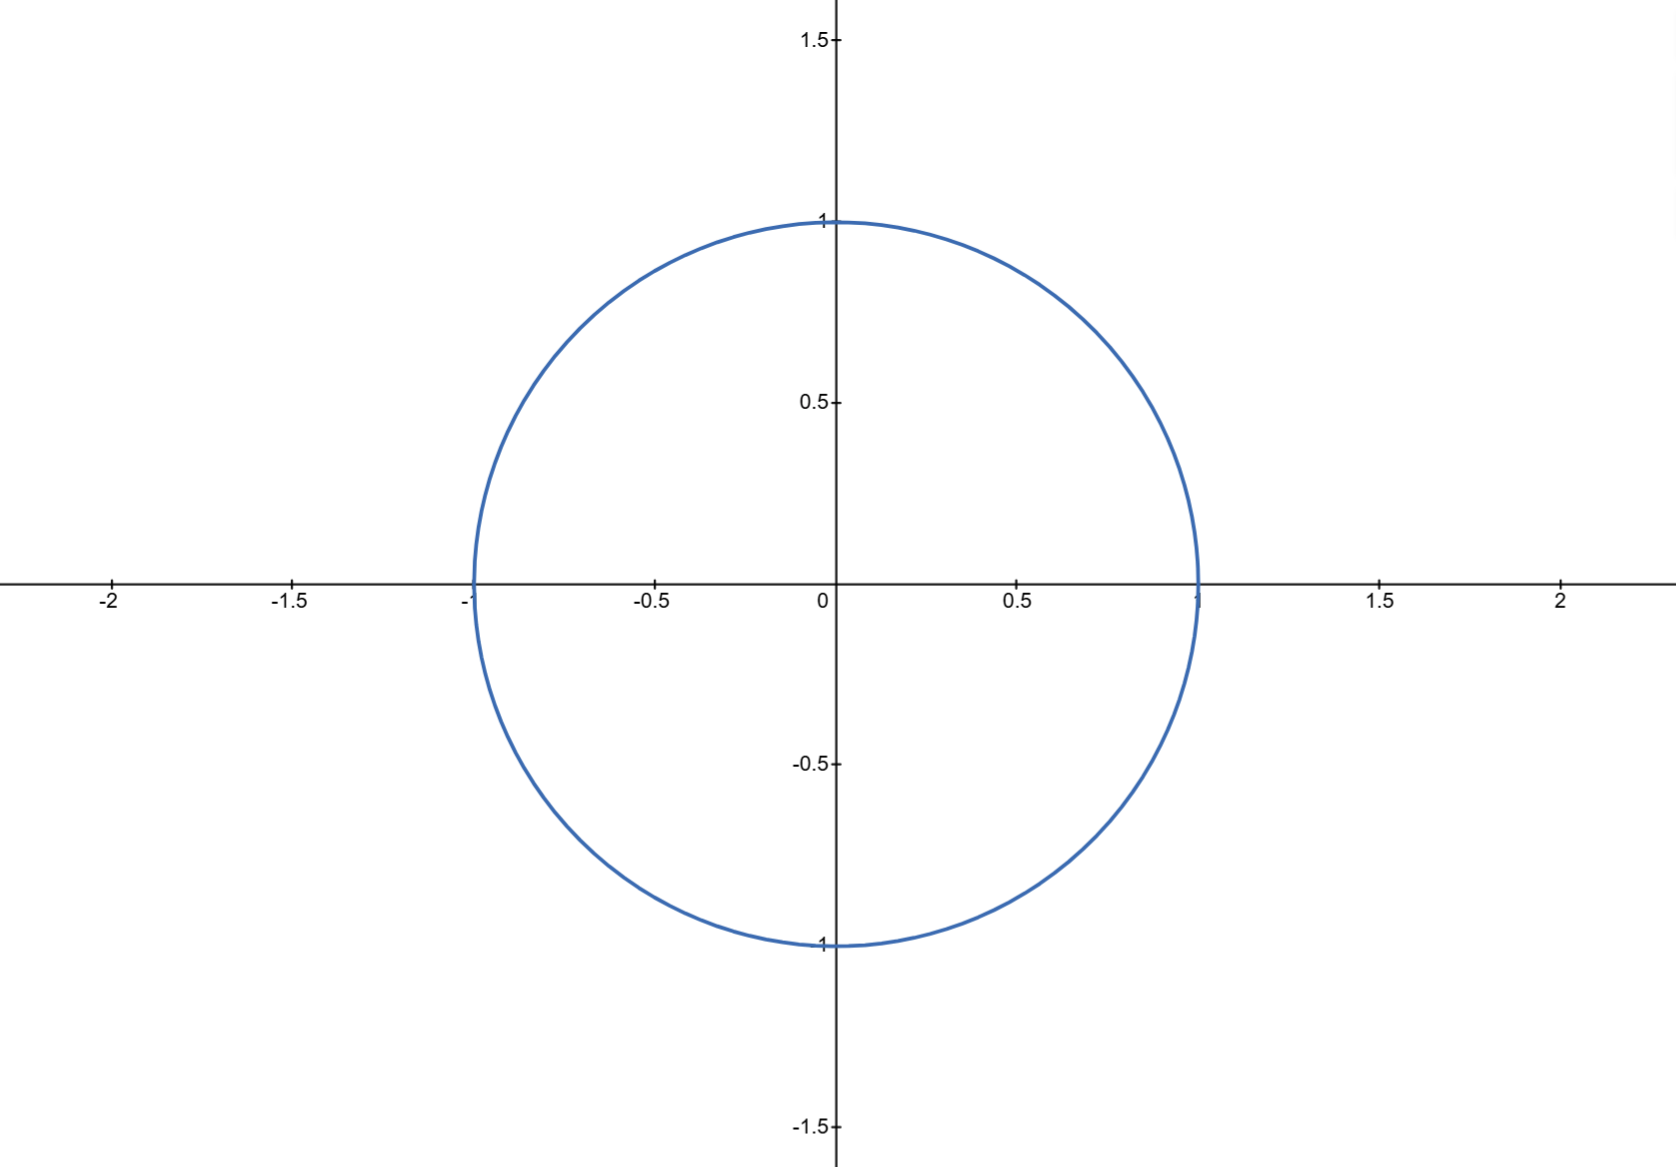
\includegraphics[width=0.6\textwidth]{img/unitCircle.png}
        \end{figure}
\end{columns}
\end{frame}


\begin{frame}{Transformaciones Afines}
Hay una definición formal de \href{https://en.wikipedia.org/wiki/Affine_transformation}{transformación afín}. Pero para nuestros propósitos, podremos decir que: una transformación afín $A: \mathbb{R}^n \rightarrow \mathbb{R}^n$ es una transformación lineal seguida de una traslación.

\begin{block}{}
    Si $\mathbf{x} \in \mathbb{R}^n$, $M$ es una matriz de $n \times n$ y $\mathbf{d} \in \mathbb{R}^n$ un vector.
    Entonces $A(\mathbf{x}) = M \mathbf{x} + \mathbf{d}$ es una transformación afín.
\end{block}
\begin{itemize}
    \item Todas las transformaciones lineales son transformaciones afines (con $\mathbf{d} = \mathbf{0}$)
    \item Todas las traslaciones son transformaciones afines (con $M = I$).
\end{itemize}
\end{frame}


\begin{frame}{Coordenadas homogéneas}

\begin{itemize}
    \item Todas las transformaciones lineales pueden llevarse a cabo multiplicando matrices.
    \item Pero las traslaciones no se pueden llevar a cabo multiplicando matrices
    \item Para solucionar ese problemas usamos las \href{https://en.wikipedia.org/wiki/Homogeneous_coordinates}{coordenadas homogéneas}
\end{itemize}
Vamos a adoptar la convención de que tanto puntos, como vectores son representados en columna.
\begin{block}{}
    Las coordenadas homogéneas de un punto $\mathbf{x} \in \mathbb{R}^n$, son una tupla de $n+1$ componentes, formada por los $n$ componentes de $\mathbf{x}$, seguidos por el escalar 1.
\end{block}
Ésta \emph{no es} la definición general, pero hará las explicaciones mas sencillas.
\begin{itemize}
    \item Las coordenadas homogéneas representan al punto $\mathbf{x} \in \mathbb{R}^n$ con un punto $\mathbf{x}_{h} \in \mathbb{R}^{n+1}$.
    \item Pero permiten \emph{expresar las transformaciones afines como una multiplicación de matrices}.
\end{itemize}

\end{frame}

\begin{frame}{Traslación}

\end{frame}

\begin{frame}{Rotación}

\end{frame}

\begin{frame}{Escalamiento}

\end{frame}

\begin{frame}{Composición de transformaciones}

\end{frame}

\begin{frame}{Operadores booleanos}
Constructive solid geometry (CSG)
\end{frame}

\begin{frame}{}
Shaders de juguete con formas complejas

Dibujar un Gato (u alguna otra figura)
\end{frame}

\begin{frame}{Raymarching}

\end{frame}

\begin{frame}{Proyección en perspectiva}

\end{frame}

\begin{frame}{Raycaster}

\end{frame}

\begin{frame}{Modelos de iluminación}

\end{frame}

\begin{frame}{Phong}

\end{frame}

\begin{frame}{Cook-Torrance}

\end{frame}

\begin{frame}{PBR}

\end{frame}

\begin{frame}{¿Cómo seguir aprendiendo?}
Pagina de Inigo quilez

Shader Book

\end{frame}
